

\section{SVJ Fit and Discovery Analysis Strategies}
\label{sec:strategies}
As was introduced in Chapter~\ref{ch:ml_tools} this analysis is interested in achieving dual goals: to make the best possible measurement of the SVJ signal model generated for this analysis, and to broadly search for any signals consistent with dark QCD behavior and inconsistent with a Standard-Model-only background hypothesis. To this end, two parallel analysis strategies are developed.\par

The SVJ Fit strategy uses the supervised PFN ML score in defining the signal region. Recall, the PFN is trained over simulated MC background and a combination of all MC SVJ signals. This gives this ML tool high sensitivity to the particular nuances of the SVJ shower predicted by the modeled theory. In addition to using the supervised ML tool, the SVJ Fit analysis strategy sets limits on the expected cross-section of each signal point in the SVJ signal grid. To achieve this, the shape of the SVJ signals are considered in the final fit, as will be elaborated on Section~\ref{subsec:fit_exclusion}. The combination of the supervised PFN ML score and the signal-shape-sensitive fitting strategy allows for the greatest possible sensitivity to the modeled signal process, thus allowing the analysis the best chance at discovery of this model, or enabling the analysis to set the best possible limits on the observed cross-section.\par

In contrast, the Discovery analysis strategy attempts to design a more general search, which could be sensitive to SVJs, but also to other possible hidden valley dark QCD models, such as fully dark jets or emerging jets \cite{snowmass}. The Discovery analysis strategy uses the semi-supervised ANTELOPE ML score in defining the signal region. Recall, the ANTELOPE is trained over ATLAS data only, with no explicit knowledge of the SVJ signal behavior. The Discovery fit strategy is also signal model agnostic, by employing a bump hunt \cite{bumphunt} strategy, which searches a smoothly falling template for any bumps inconsistent with a background only hypothesis. Therefore any signal which could present a resonant signature in \mt~could show up as an excess in this strategy. \par

The details of both strategies will be explored in the follow sections which detail the design of the signal regions and fit strategies.
A diagram demonstrating the analysis flows can be seen in Figure~\ref{fig:analysisflow}.
Details on each selection and region can be found in the following subsections.
\begin{figure}[!htbp]
\centering
    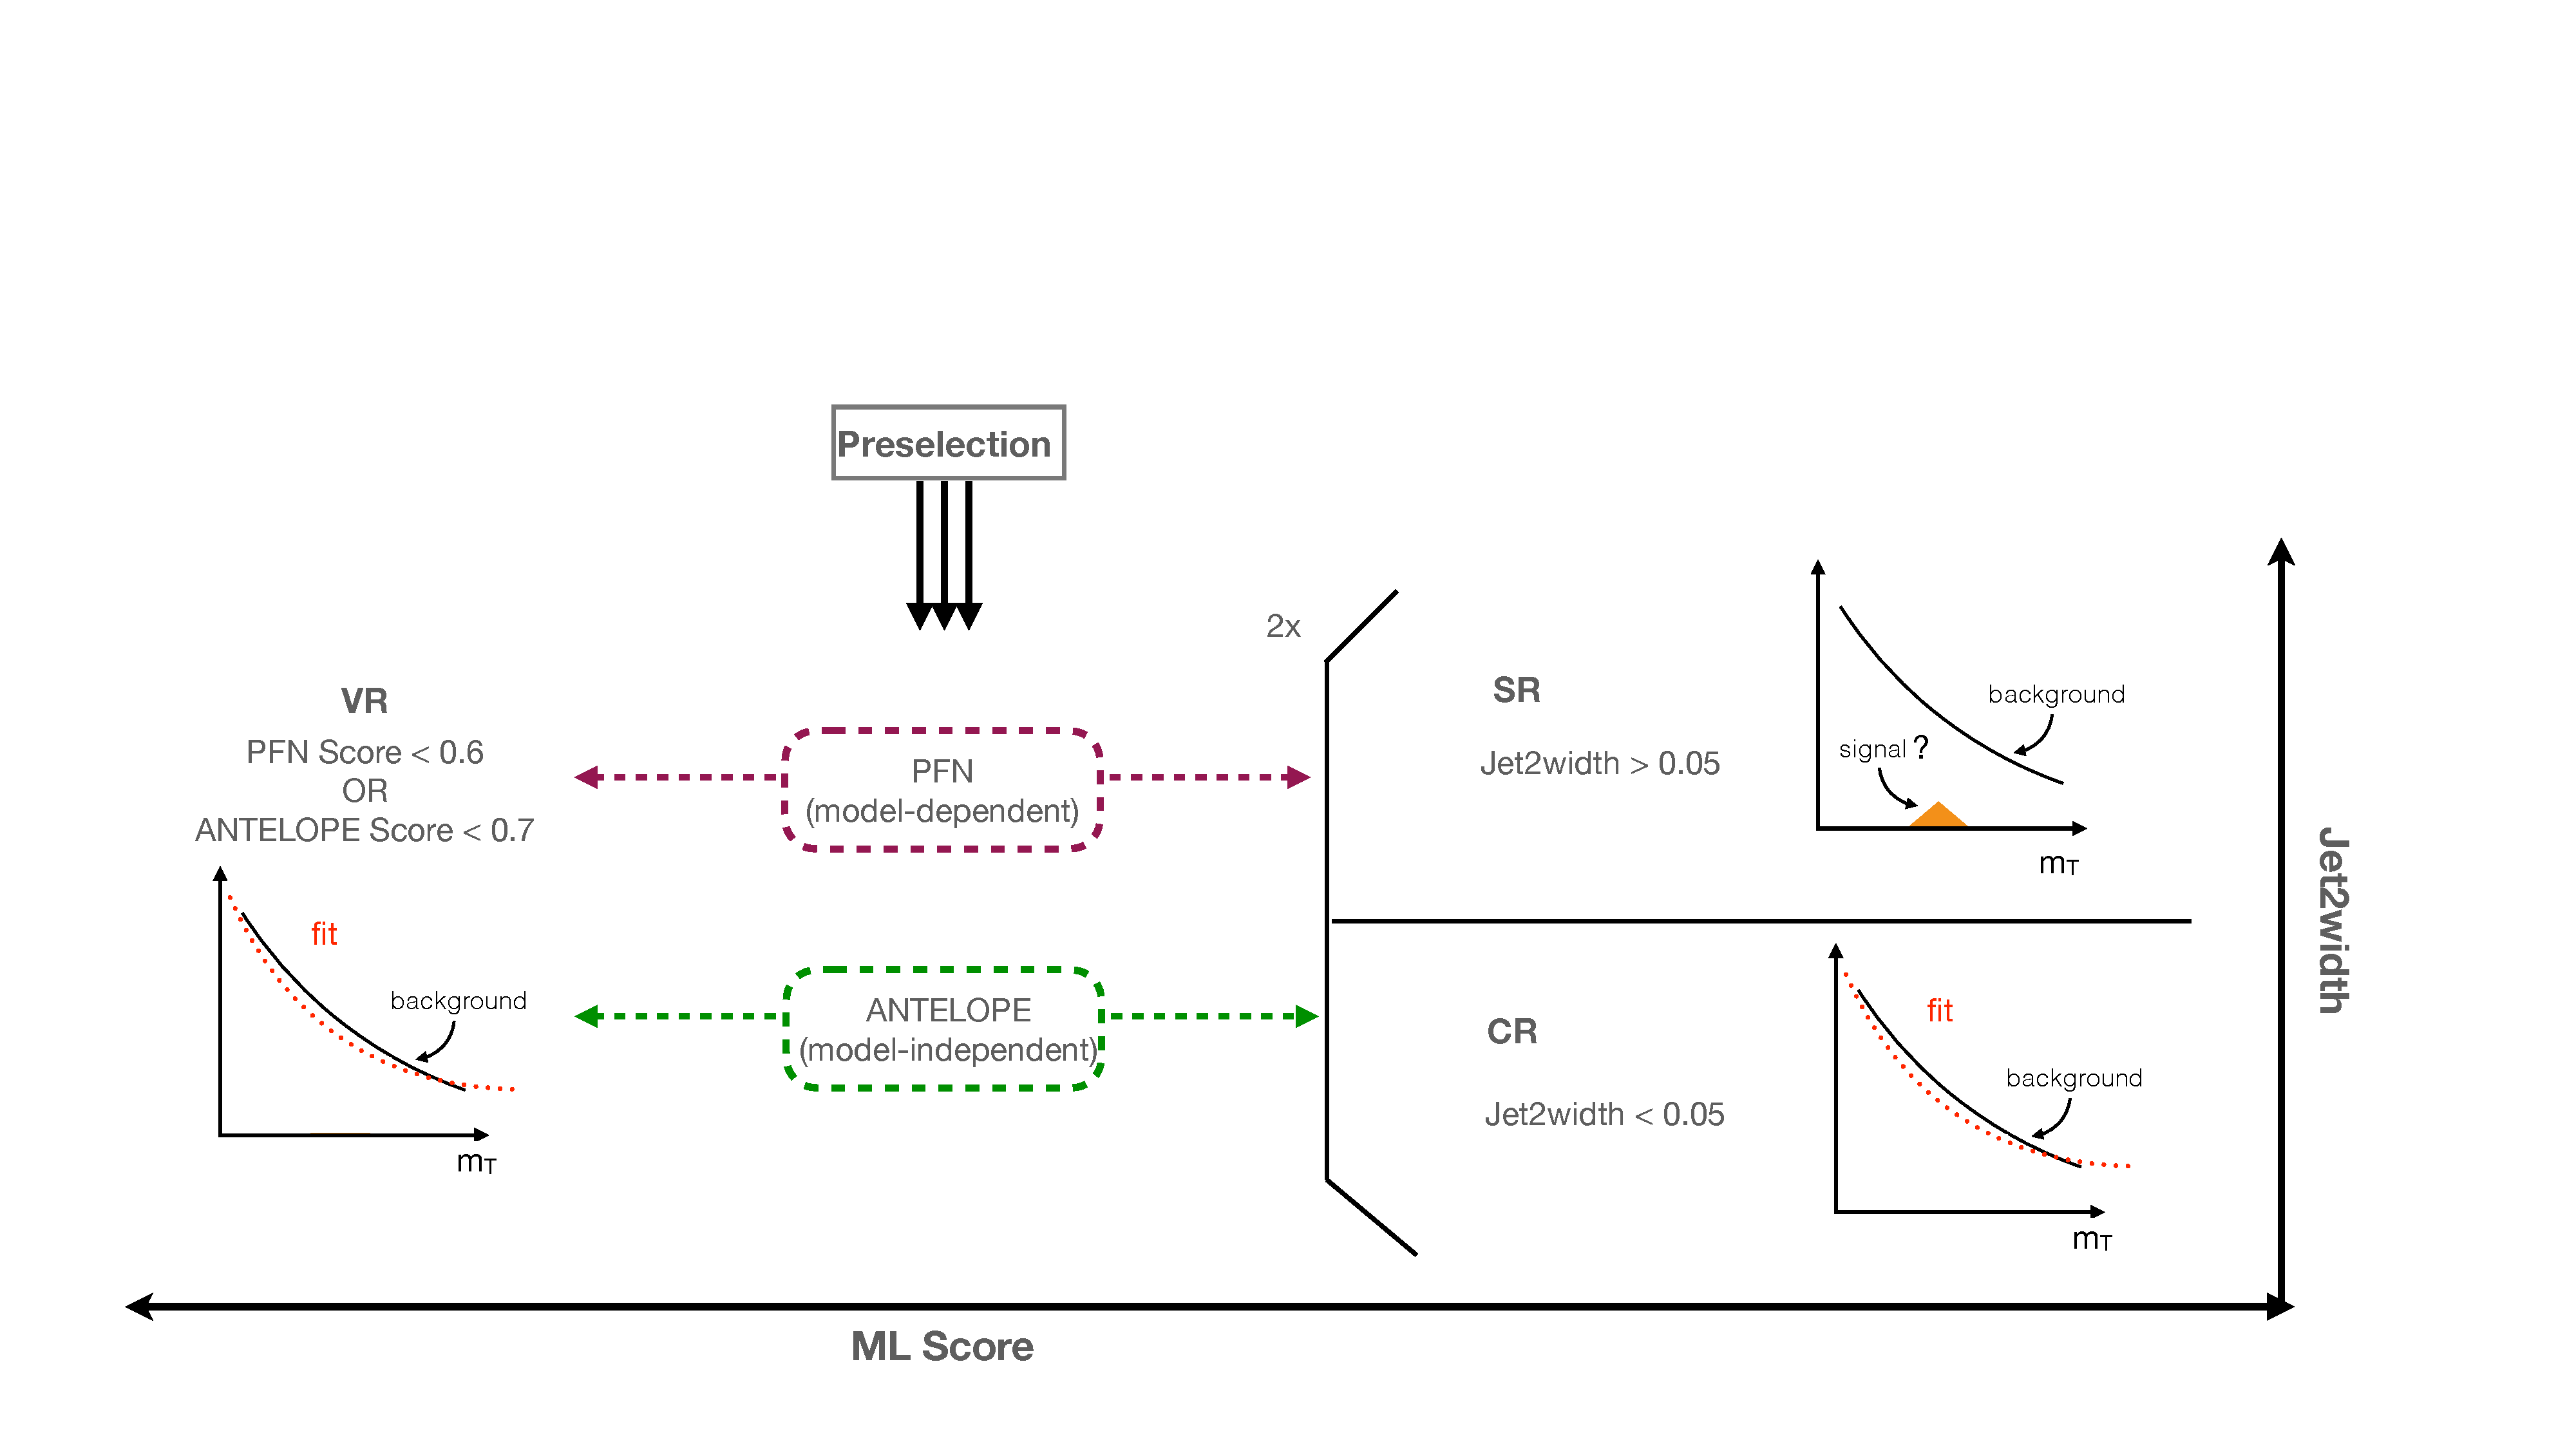
\includegraphics[width=1.1\textwidth]{figures/eventsel/analysisflow_vr}
    \caption{Flow of analysis selections, regions, and background estimation/validation fitting strategy.
    \label{fig:analysisflow}}
\end{figure}

\section{Analysis Regions}
%------------------------------------------------- 
\subsection{Control and Validation Regions}
\label{subec:sel_crvr}

The final background estimation will come from a polynomial fit to the \mt~ distribution in the signal region.
The control and validation regions are needed to develop and test this fit in data.
 
To define the CR selection, a variable is needed that isolates background from all signals across the (\rinv, $m_Z$) grid, which is challenging due to the varying nature of the signal models in quantities such as \met~ and \pt~balance, as illustrated in Figure~\ref{fig:presel_vars}. 
The variable \textit{jet width} is chosen, which is the calorimeter measurement of the width of a small-R jet as defined by the distance between the cluster and the jet axis scaled by the jet energy~\cite{jetwidth}.
Figure~\ref{fig:jet2width} shows this variable specifically for the subleading jet width, both in data vs. MC at preselection, and for background vs. signals, indicating this broad discrimination power.
The leading jet width, which was determined to be less useful for isolating signal from background is also shown.
The subleading jet is more likely to be the jet aligned with MET, which is why the signal jet width is consistently wider in the subleading jet, but not the leading jet.  %, using v12 of the ntuples.
A selection of \textbf{jet2width $<$ 0.05} is chosen for the CR, with the VR and SR therefore having a selection of jet2width $>$ 0.05.
TODO: put diff jet2width plot here, remove from presel
 
\begin{figure}[!htbp]
\centering
   %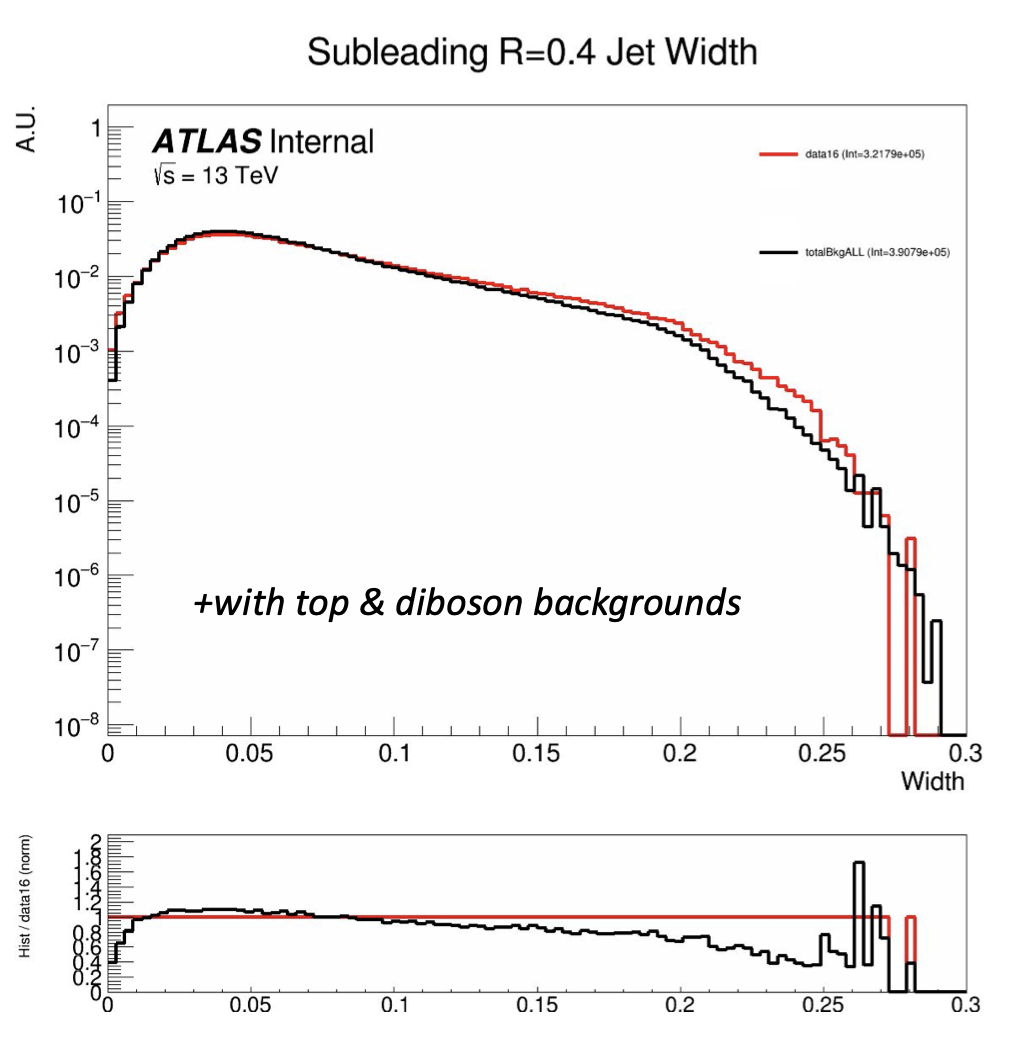
\includegraphics[width=0.4\textwidth]{figures/background/jet2width_datamc}
   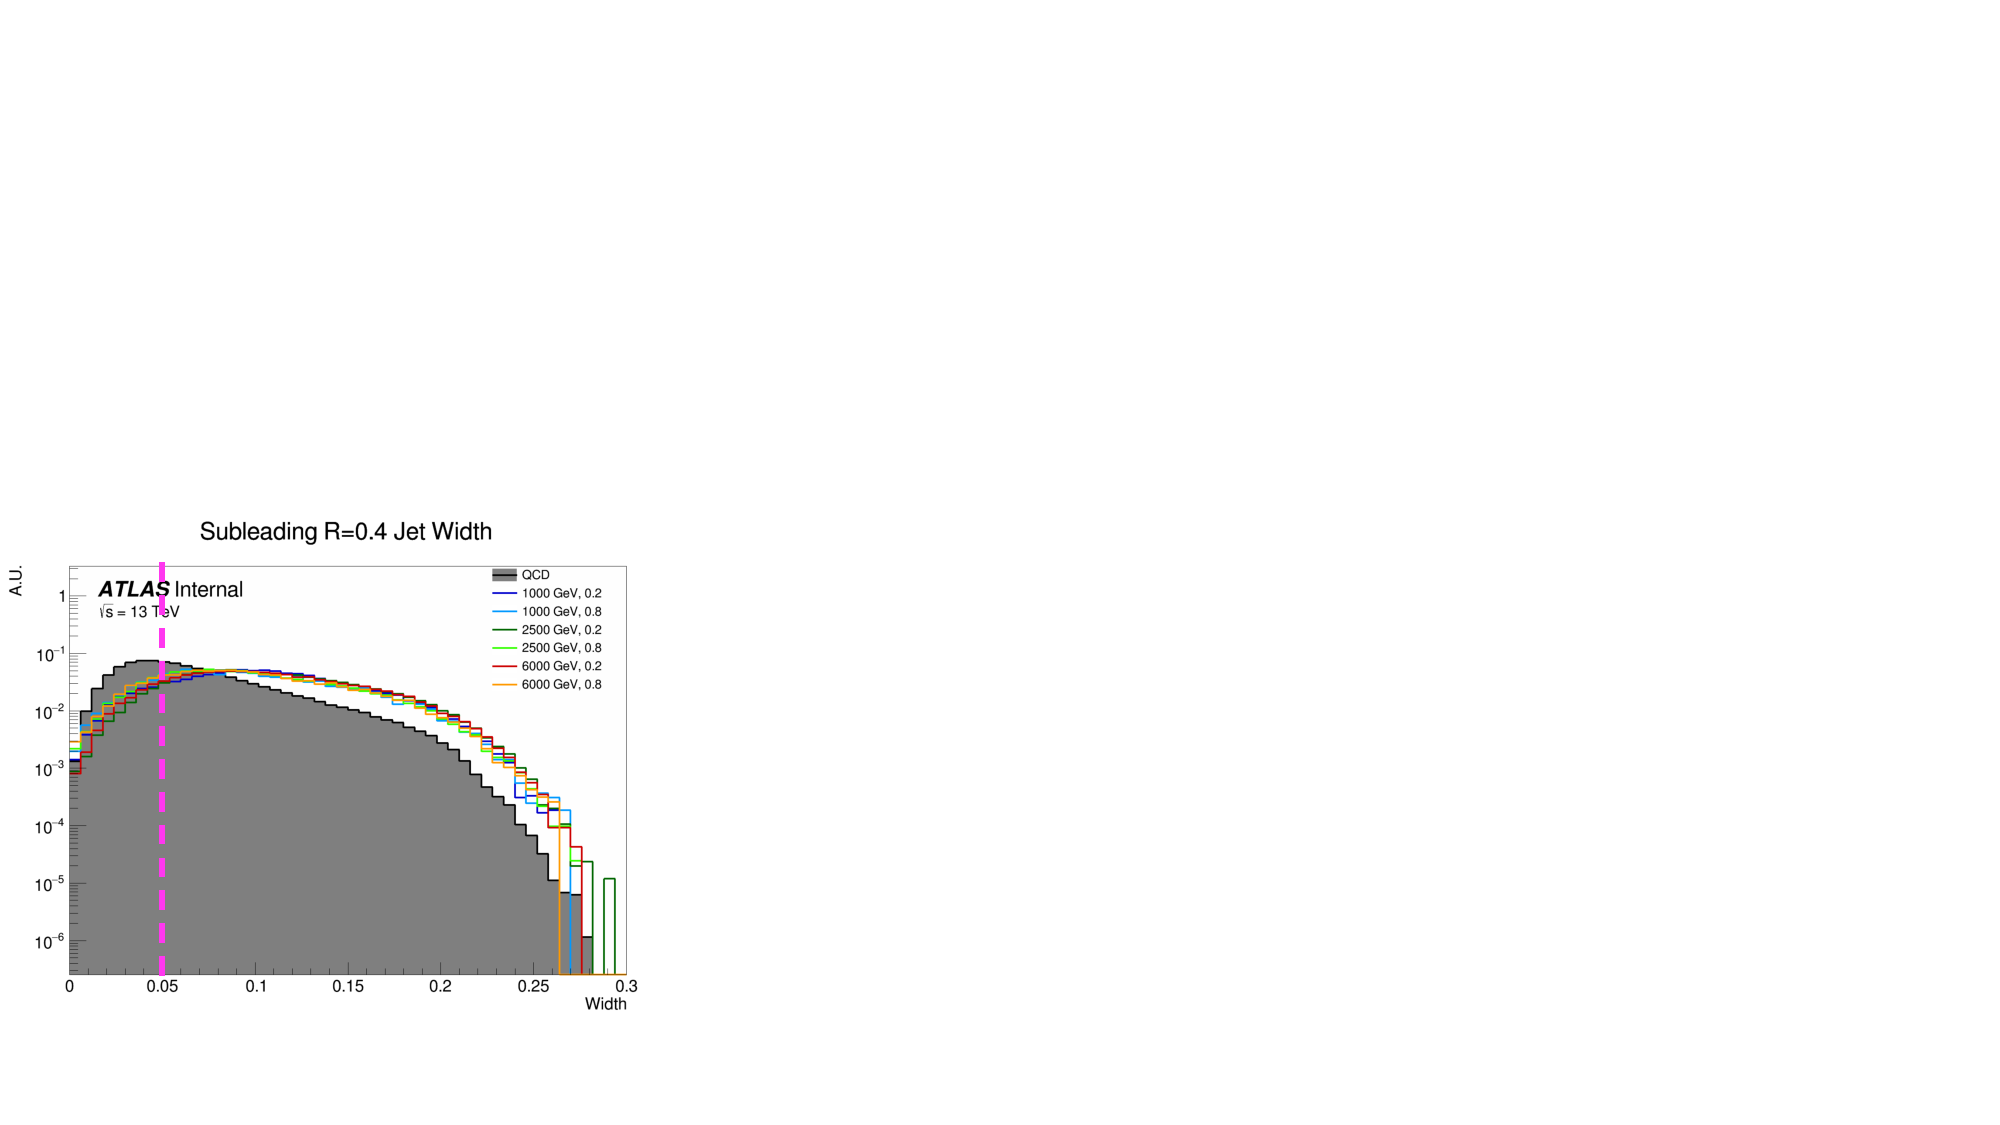
\includegraphics[width=0.45\textwidth]{figures/background/jet2width}
   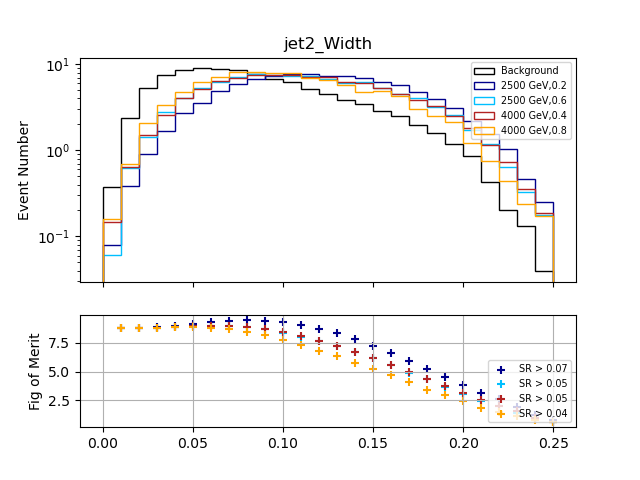
\includegraphics[width=0.45\textwidth]{figures/background/jet2width_bkgsignal}
    \caption{Distributions of the subleading jet width \textbf{jet2width} in data vs. background MC and signals at preselection (left) and background vs. representative signal models following the PFN score selection (right). Background MC comprises the samples listed in Appendix~\ref{app:mcsamples}. Demonstrates that jet2width remains a discriminating variable after ML tool selection is made.
    \label{fig:jet2width}}
\end{figure}

While the CR was used to develop the polynomial strategy, and is the primary region used in many of the fit studies, a validation region is used as an additional check of the estimation strategy in data.
The VR is defined using the region of events with low ML score by either the PFN or ANTELOPE networks.
Here the analysis strategy splits into the two parallel strategies presented in Section~\ref{sec:stragies}: the SVJ fit strategy and the dis
A selection of textbf{PFN score $\leq$ 0.6 \& jet2width $\geq$ 0.05} defines the SVJ fit VR, while textbf{ANTELOPE score $\leq$ 0.7 \& jet2width $\geq$ 0.05} defines the discovery VR. 

There are therefore three variables that are crucial to the analysis strategy: \textbf{jet2width, PFN/ANTELOPE score, and \mt}.
Figure~\ref{fig:bkg_correlations} shows the correlations of all three variables to one another.
Any outstanding correations are shown in Figure~\ref{fig:crvrsr_mt} to not sculpt the \mt~distribution and only affect its slope, making these variables trustworthy for extrapolation across background/signal regions and final fitting procedures.
\begin{figure}[!htbp]
\centering
   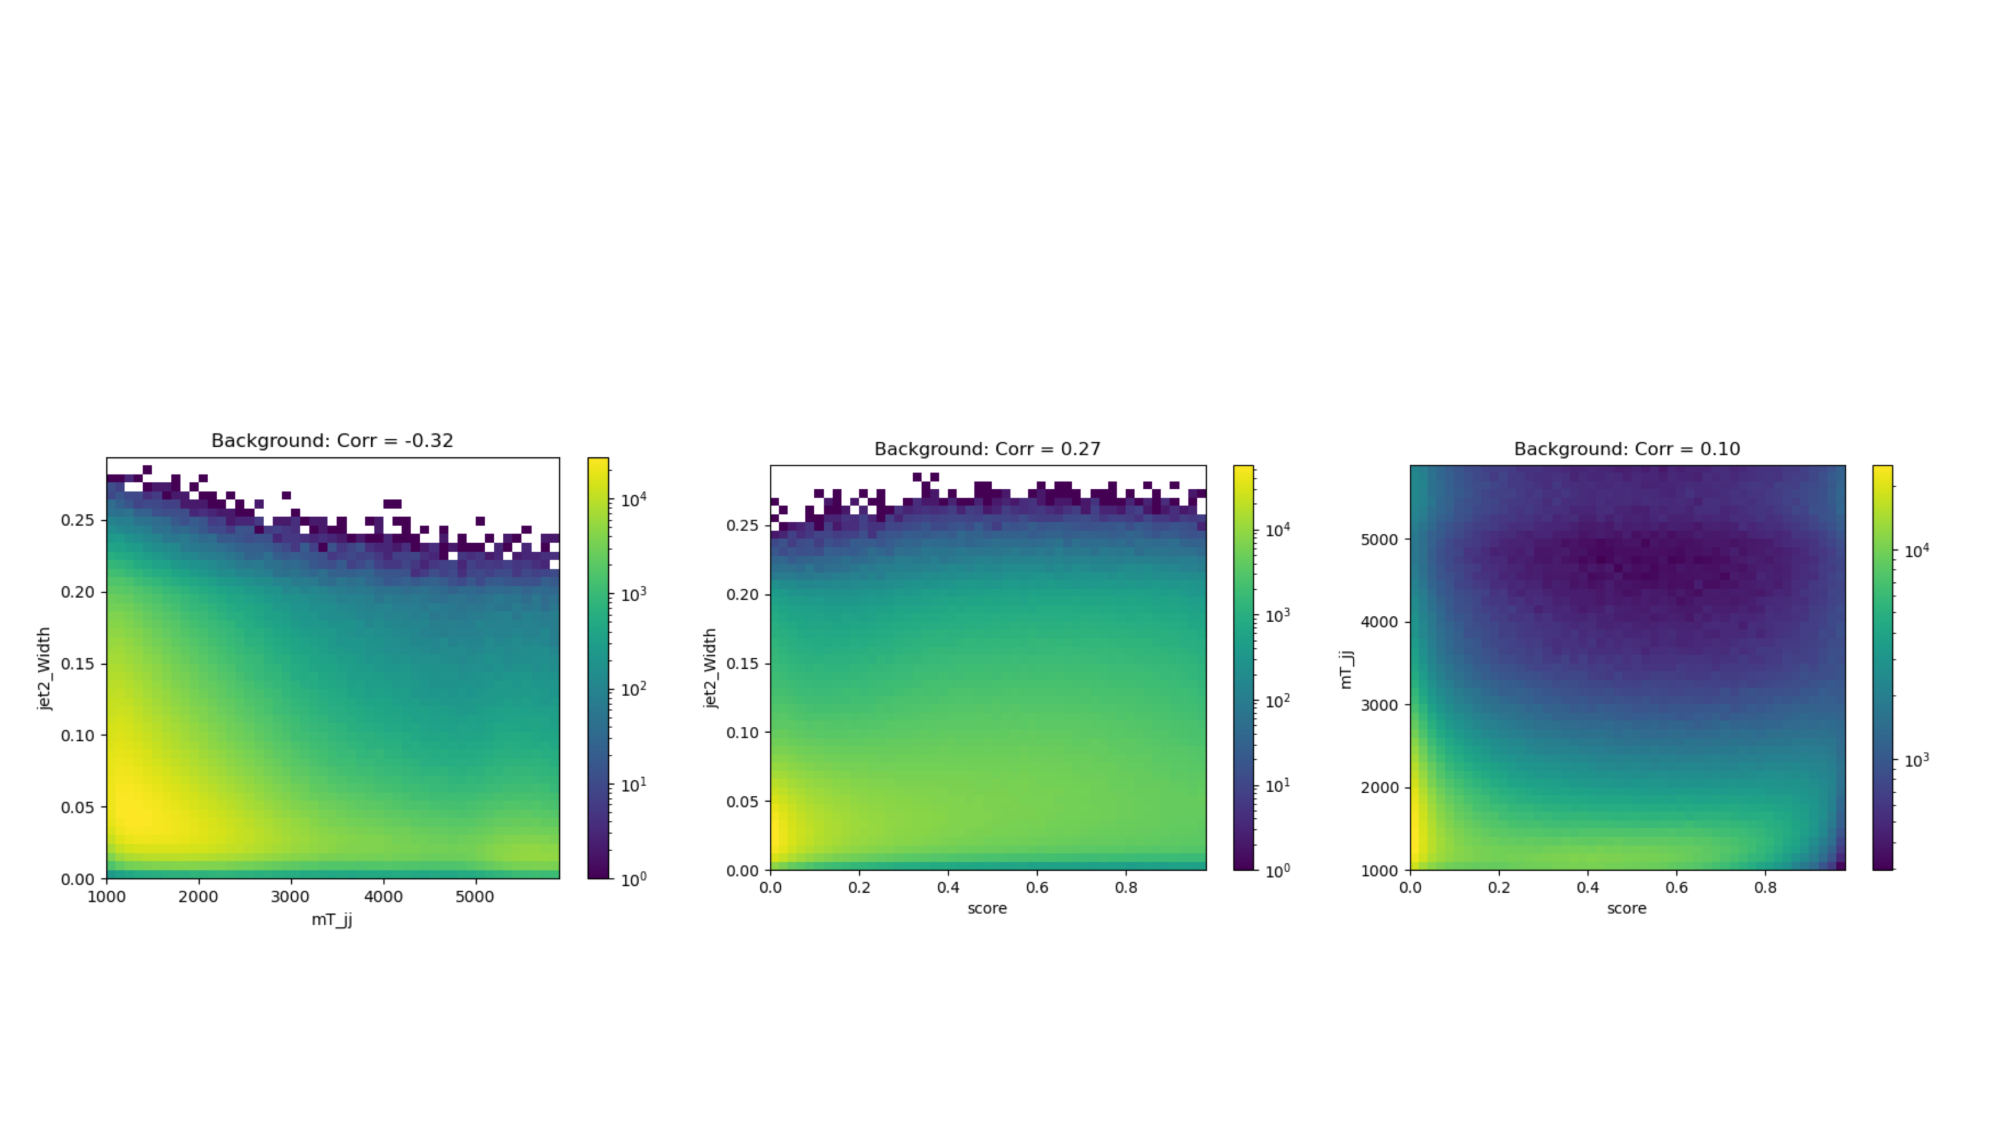
\includegraphics[width=0.95\textwidth]{figures/background/bkg_correlations}
   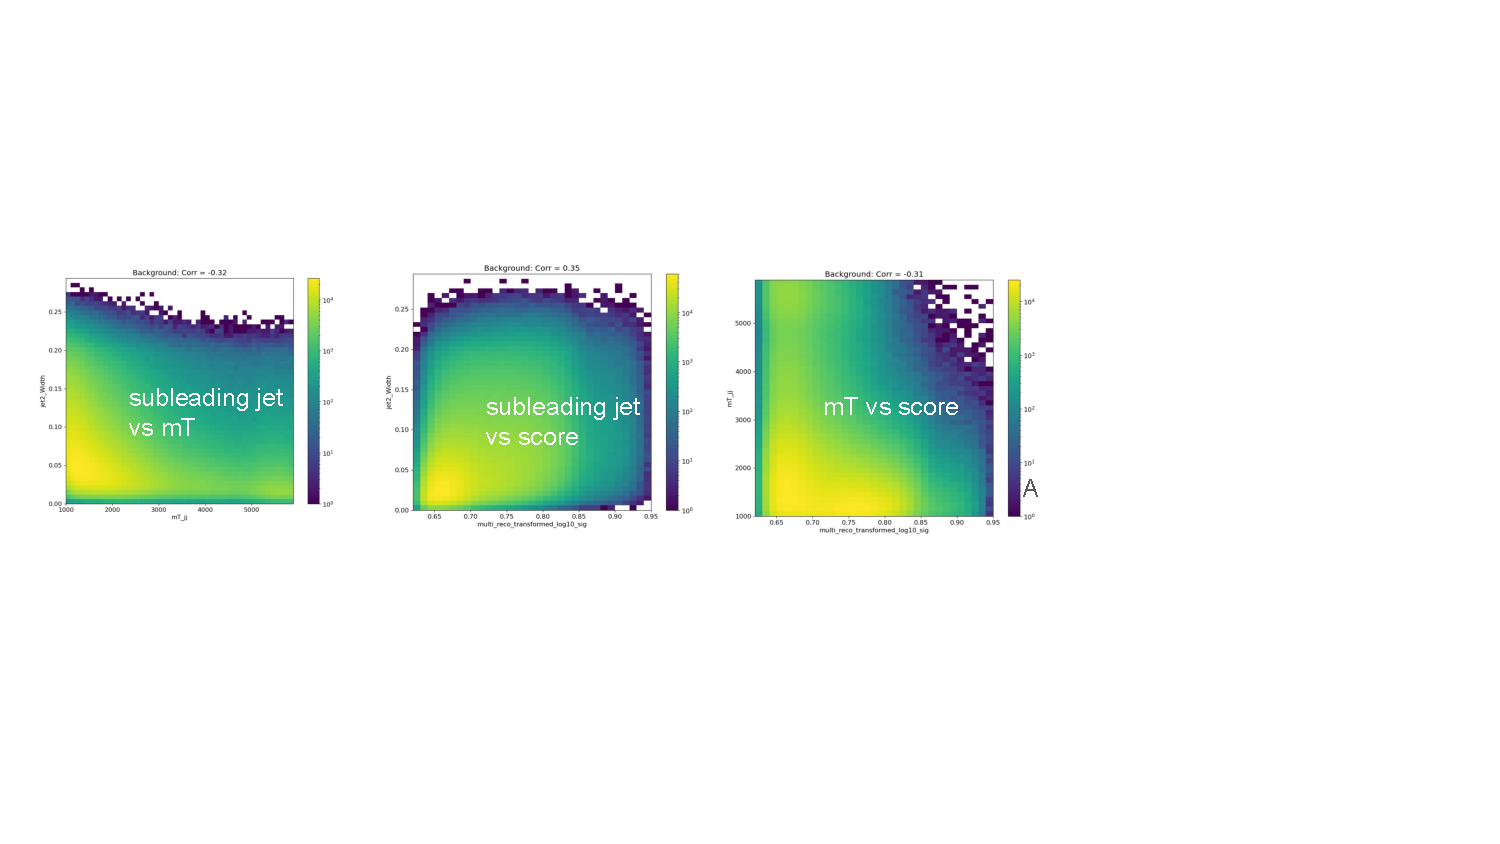
\includegraphics[width=0.95\textwidth]{figures/background/bkg_correlations_antelope}
    \caption{2D plots revealing correlations between jet2width and \mt~(left), jet2width and ML score (middle), and \mt~with ML score (right). For the top row, the ML score is the PFN score, and for the bottom three, the ML score is the ANTELOPE score. Minimal correlations are observed and are shown to not sculpt \mt, validating these variables for analysis region construction and statistical treatment.
    \label{fig:bkg_correlations}}
\end{figure}

The most important variable for shape robustness across the CR, VR, and SR is \mt, as this is the variable that is fit for the statistical results.
Figure~\ref{fig:crvrsr_mt} shows the distribution of \mt~across the CR, VR, and SR, for both the PFN (supervised) and ANTELOPE (semi-supervised) strategies.
Some slope is observed in the ratio of the CR to the VR/SR shapes; however, the chosen background estimation strategy of polynomial fitting is expected to accommodate this slope.
Further, the ability of the background polynomial to fit both tail shapes will flex the fit framework in a way that will generate higher confidence in the final ability to fit the SR.
No significant bumps or sculpting are observed.%, which could be more problematic for a bump-hunt analysis.
\begin{figure}[!htbp]
\centering
   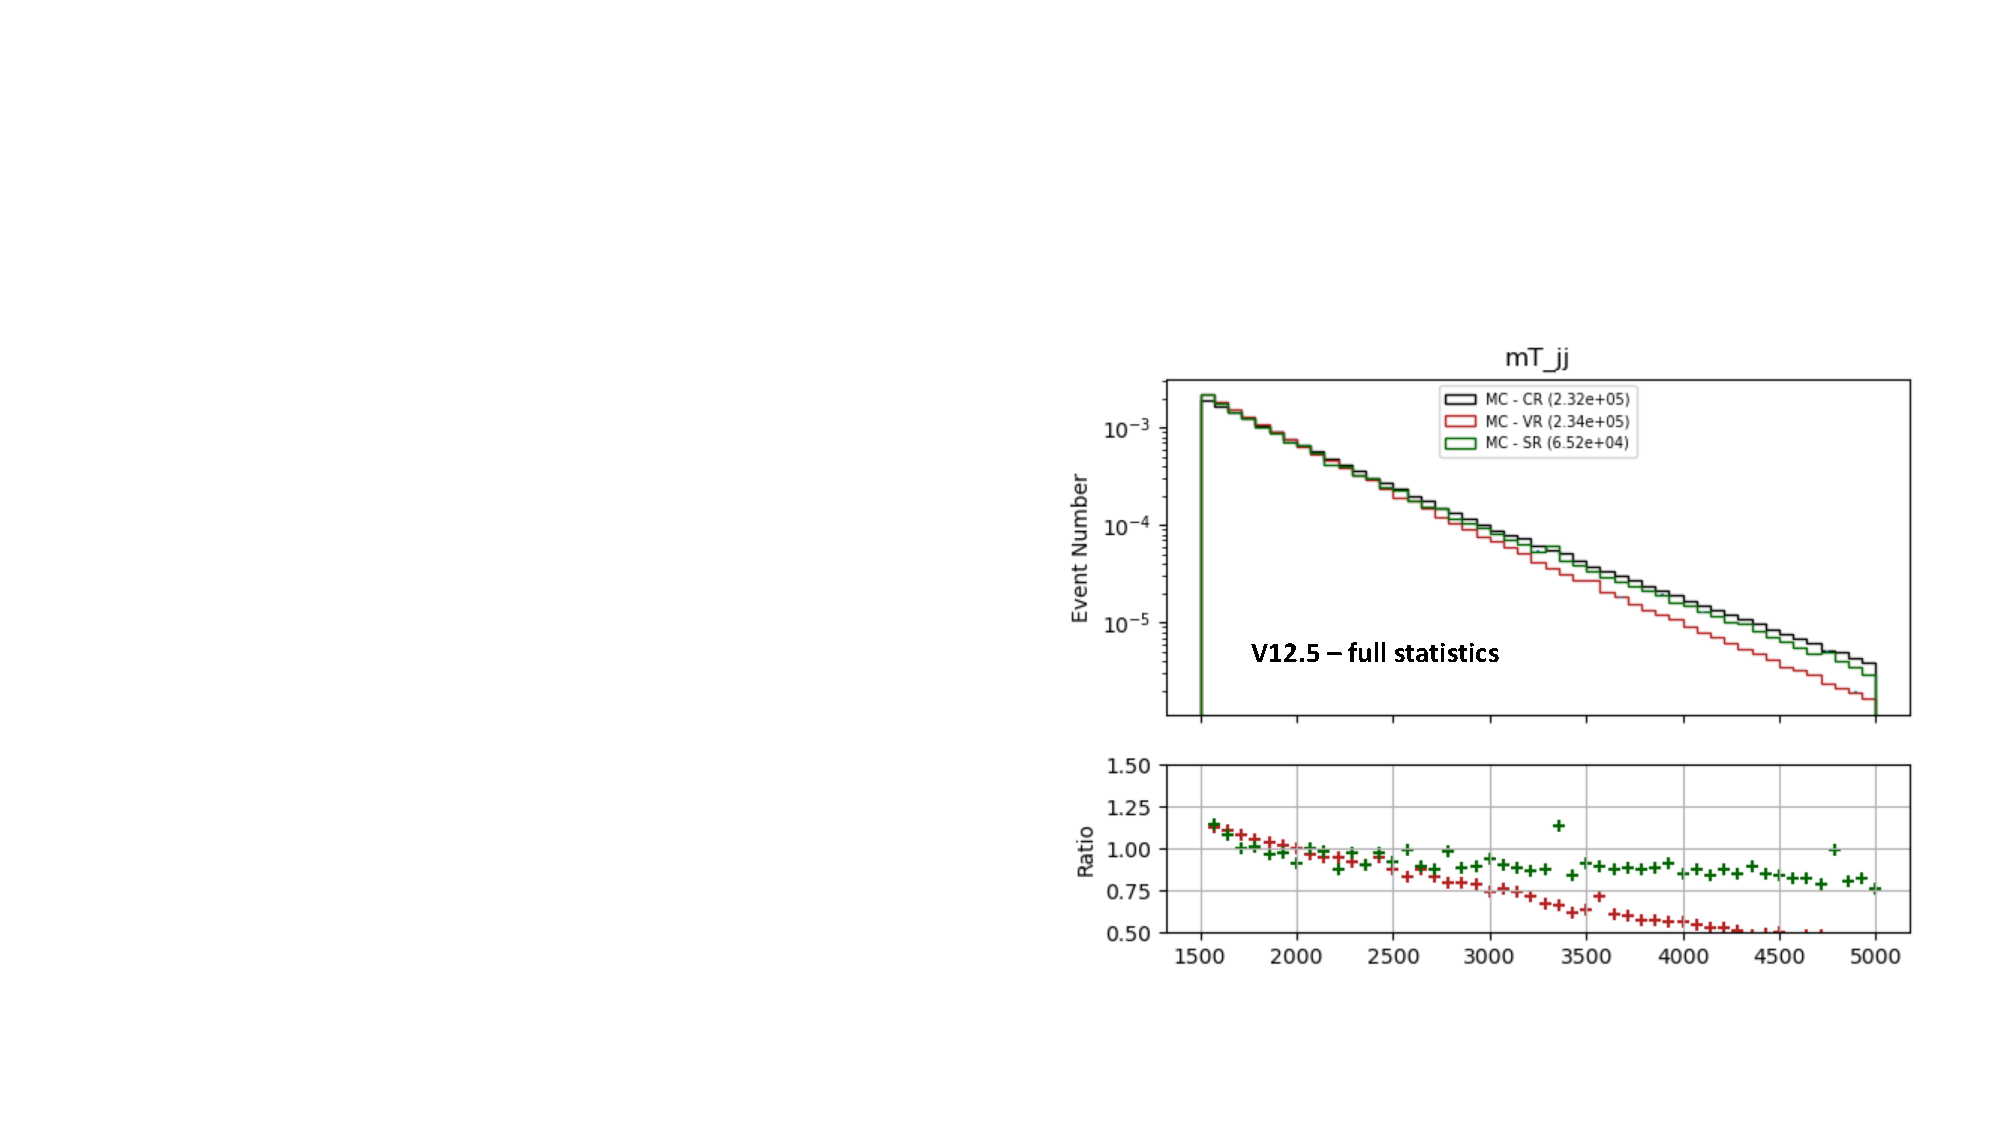
\includegraphics[width=0.45\textwidth]{figures/eventsel/PFN_mT_regions}
   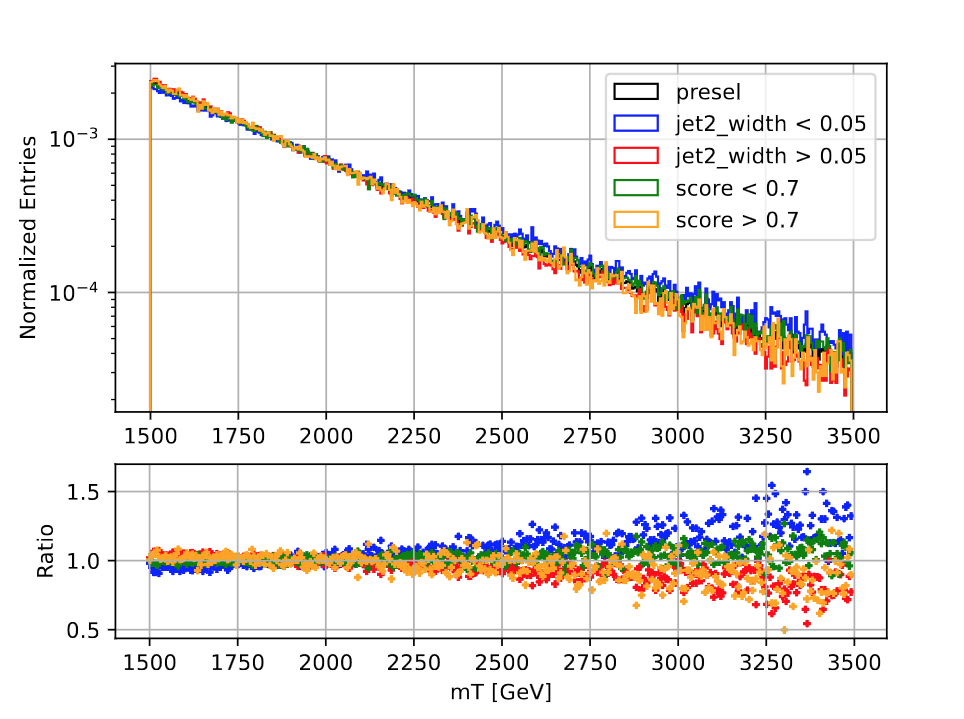
\includegraphics[width=0.45\textwidth]{figures/eventsel/antelope_mT_regions}
    \caption{\mt~in simulation across the CR, VR, and SR for both PFN (left) and ANTELOPE (right) selections. 
    \label{fig:crvrsr_mt}}
\end{figure}

Plots of the $\phi$ shape variables in the CR and VR, and correlations of these variables with ML score are available in Appendix~\ref{app:pfn_var_corr}. 


%------------------------------------------------- 
\subsection{Signal Region}
\label{subec:sel_sr}

A selection of \textbf{PFN score $>$ 0.6} (\textbf{ANTELOPE score $>$ 0.7}) is made to provide the primary signal-to-background enrichment, as motivated by Section~\ref{subsec:supervised}.
Subsequently, the selection of \textbf{jet2width $>$ 0.05} is made to enrich signal across the (\rinv, $m_Z$) grid and orthogonalize the SR to the CR.
Note that the PFN and ANTELOPE regions are not orthogonal; this is because the two analysis flows serve different purposes, their statistical treatments are different, and they will not be combined. 

A summary of the SR, CR, and VR definitions can be seen in Figure~\ref{fig:crvrsr_2d}, along with the relative data statistics in each region.
\begin{figure}[!htbp]
\centering
    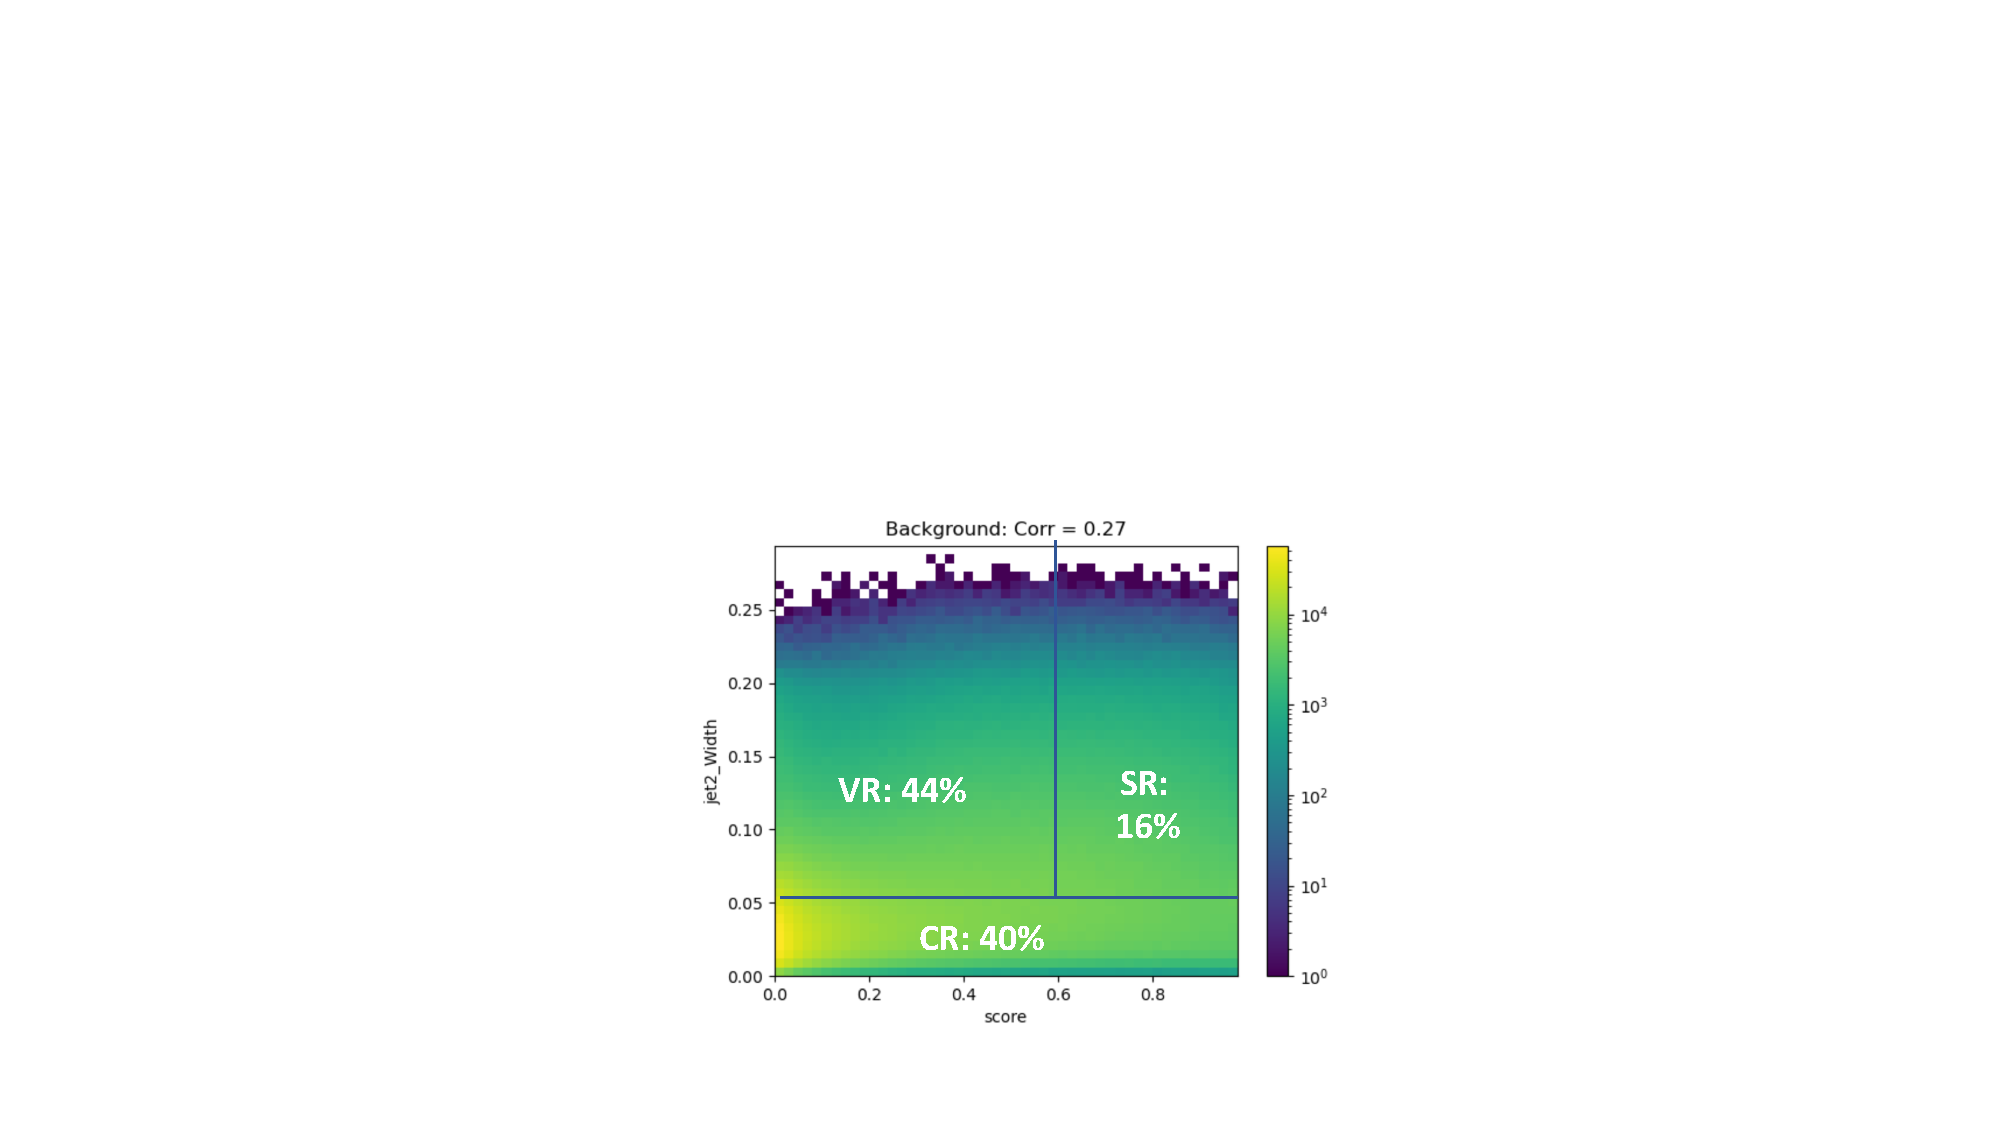
\includegraphics[width=0.6\textwidth]{figures/eventsel/crvrsr_2d}
    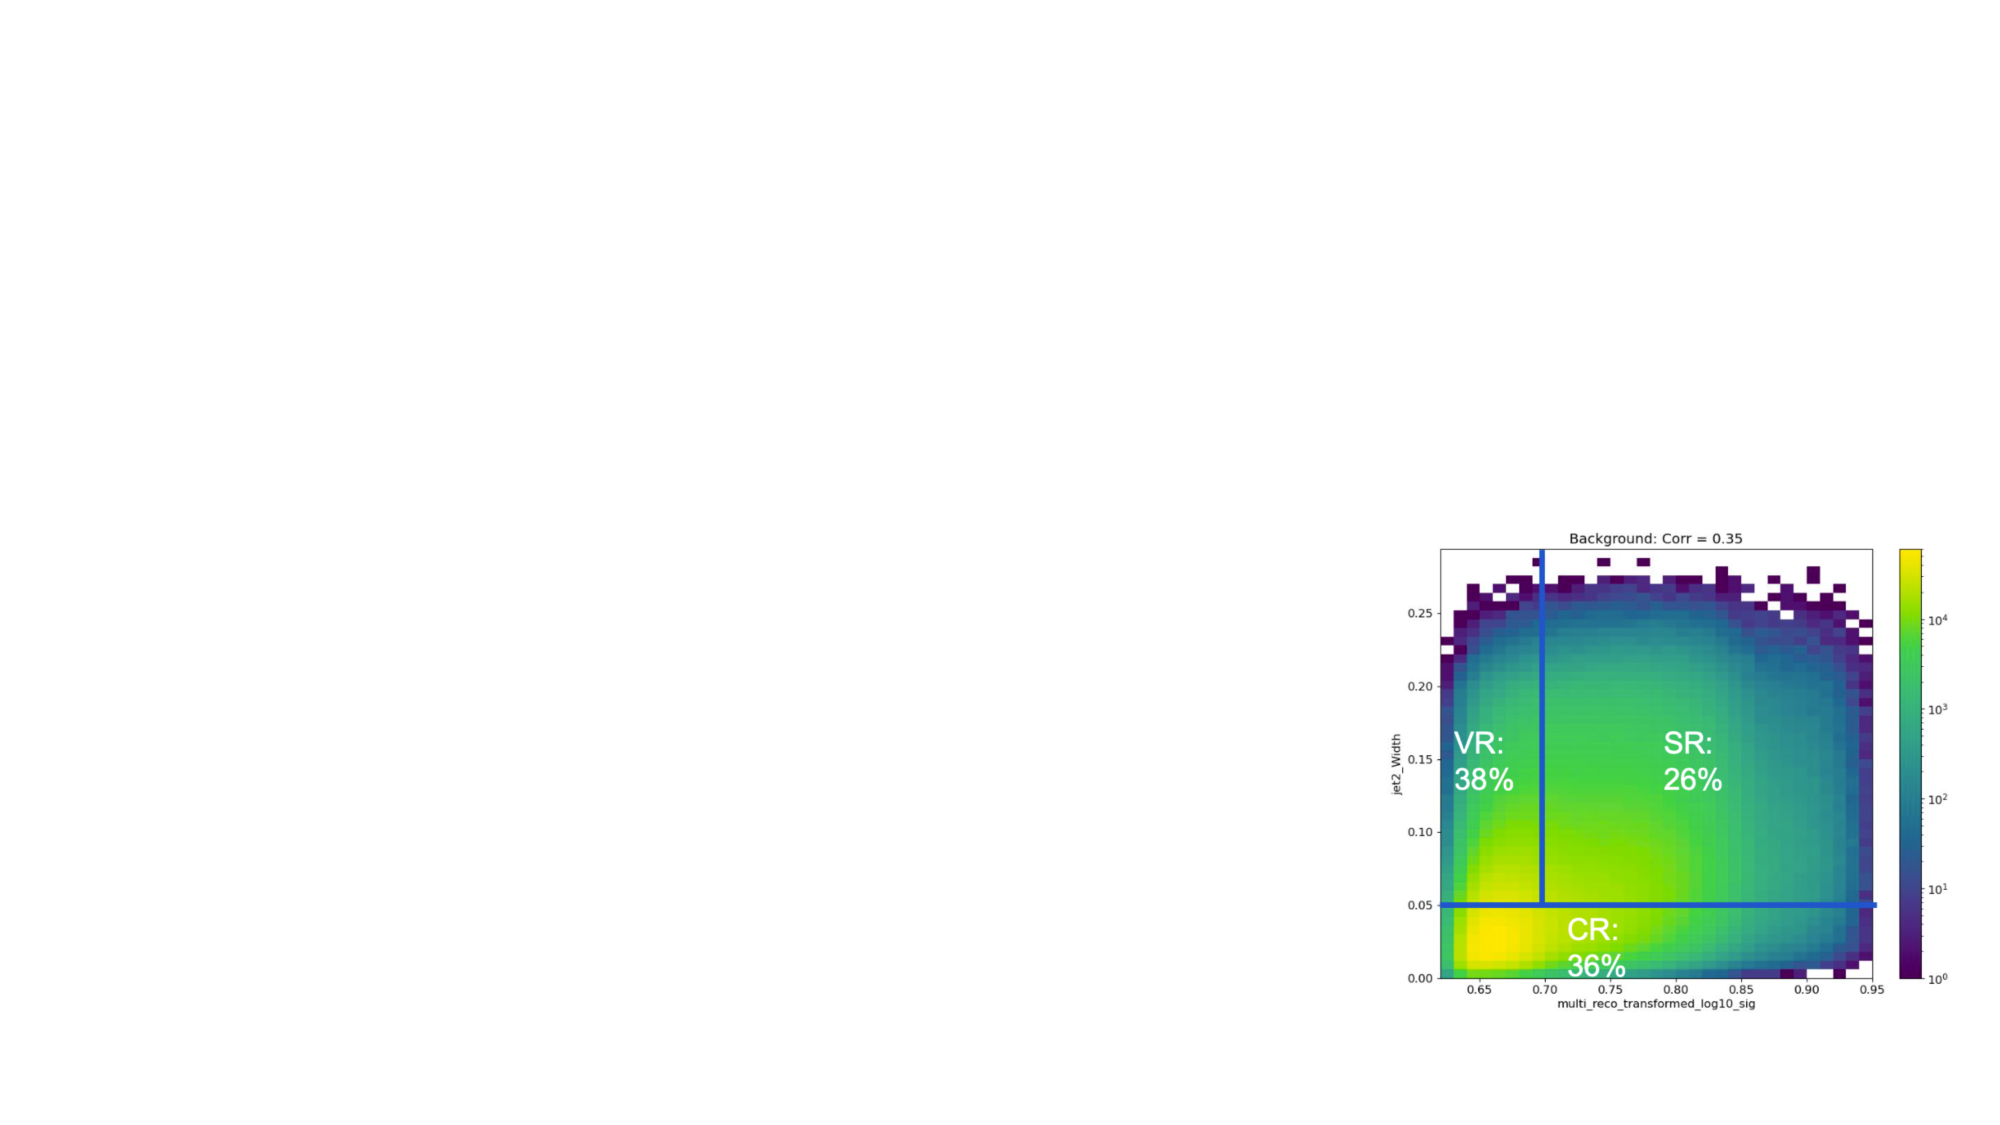
\includegraphics[width=0.6\textwidth]{figures/eventsel/crvrsr_2d_antelope}
    \caption{Definition of CR, VR, and SR regions using \textsc{jet2width} and the PFN score, along with the population of each region in data statistics for the PFN (top) and ANTELOPE (bottom) analyses. 
    \label{fig:crvrsr_2d}}
\end{figure}



